\section*{Problem 1 - Attitude Control of Satellite}

The objective of problem 1 is to control attitude of a satellite. The satellites equations of motions are represented in equation \eqref{eq:dynamics},  \cite{Fossen2011}. The parameters for this specific satellite are; $\mathbf{I}_{CG} = mr^2$, $m = 100 kg$, $r = 2.0 m$.  

\begin{subequations}
\label{eq:dynamics}
	\begin{align}
		\dot{\mathbf{q}} = \mathbf{T}_q (\mathbf{q} ) \boldsymbol{\omega} \\
		\mathbf{I}_{CG} \dot{\boldsymbol{\omega}} - \mathbf{S} (\mathbf{I}_{CG} \boldsymbol{\omega} ) \boldsymbol{\omega} & =  \boldsymbol{\tau} 
		\label{eq:EOM_omega_dot}
	\end{align}	
\end{subequations}

These equations uses the unit quaternions and Euler angles. The unit  quaternions are represented as $q = [\eta, \epsilon_1, \epsilon_2, \epsilon_3]^\top$ and only the positive $\eta$ is used, leading to equations \eqref{eq:pos_eta}. The Euler angles are represented as $\theta = [\phi , \theta , \psi]^\top$ and their representative angular velocities are  $\omega = [\omega_1, \omega_2, \omega_3]$. In \cite{Fossen2011} $\omega$ is often written as $\omega = [p,q,r]$, but because of the parameter $r = 2.0m$, in this rapport $\omega$ is written as $[\omega_1, \omega_2, \omega_3]^\top$.

\begin{equation}
    \eta = \sqrt{1 - \epsilon^\top \epsilon} 
    \label{eq:pos_eta}
\end{equation}
 
In this lab report the state of the system $x = [ \boldsymbol{\epsilon}^\top, \boldsymbol{\omega}^\top]$ and the input to the system $\mathbf{u} = \boldsymbol[0,0,0,\tau_1, \tau_2, \tau_3]^\top$. The reason for the upper three zeros in the input, is because of $\dot{\boldsymbol{\epsilon}}$ do not have any input, while $\dot{\boldsymbol{\omega}}$ have input $\boldsymbol{\tau}$.

\subsection*{Problem 1.1}

\subsubsection*{Finding the equilibrium point}

The equilibrium point is defined as the steady-state solution of a system, meaning $\dot{\mathbf{x}} = 0$ and $\mathbf{u}= \mathbf{0}$. \todo{Enig Alexandra ? }

The equilibrium point $\mathbf{x_0}$ of the closed-loop system $\mathbf{x} = [ \boldsymbol{\epsilon}^\top, \boldsymbol{\omega}^\top]^\top$ corresponding to $\mathbf{q} = [\eta,\epsilon_1, \epsilon_2, \epsilon_3]^\top = [1, 0, 0, 0]$ and $\boldsymbol{\tau} = \boldsymbol{0}$ may be found by setting $\dot{\boldsymbol{\epsilon}} = \mathbf{0}$ and $\dot{\boldsymbol{\omega}} = \mathbf{0}$. The equation for $\boldsymbol{\epsilon}$ and $\boldsymbol{\omega}$ may be found by using equation (2.86) in \cite{Fossen2011} and \eqref{eq:EOM_omega_dot}. From equation (2.86) in \cite{Fossen2011} and \eqref{eq:EOM_omega_dot} the following equations were found:

\begin{subequations}
\label{eq:x_dot}
	\begin{align}
		\dot{\boldsymbol{\epsilon}} =  [ \eta \mathbf{I}_{3X3} + \mathbf{S}(\boldsymbol{\epsilon}) ] \boldsymbol{\omega}  \label{eq:episilon_dot} \\
		 \dot{\boldsymbol{\omega}} = \mathbf{I}_{CG}^{-1} [\mathbf{S} (\mathbf{I}_{CG} \boldsymbol{\omega} ) \boldsymbol{\omega} +  \boldsymbol{\tau} ] \label{eq:omega_dot}
	\end{align}	
\end{subequations}


With skew-matrices $\mathbf{S} (\boldsymbol{\epsilon})$ and $\mathbf{S} (\mathbf{I}_{CG} \boldsymbol{\omega} ) $, as defined in \cite{Fossen2011} equation (2.10). Equation \eqref{eq:episilon_dot} may be written as:


\begin{equation}
    \begin{aligned}
	\dot{\boldsymbol{\epsilon}}
	&= 
	\left \{
	\begin{bmatrix}
		\sqrt{1-\boldsymbol{\epsilon}^\top \boldsymbol{\epsilon}} & 0 &  0  \\
		0 & \sqrt{1-\boldsymbol{\epsilon}^\top \boldsymbol{\epsilon}} &   0   \\
		0 &  0  & \sqrt{1-\boldsymbol{\epsilon}^\top \boldsymbol{\epsilon}} 
	\end{bmatrix}
	+
	\begin{bmatrix}
		0 & -\epsilon_3 &  \epsilon_2   \\
		\epsilon_3 & 0 &   - \epsilon_1   \\
		-\epsilon_2 &  \epsilon_1  & 0
	\end{bmatrix}
	\right \} 
	\begin{bmatrix}
		\omega_1  \\
		\omega_2  \\
		\omega_3  \\
	\end{bmatrix}
	\end{aligned}
	\label{eq:epsilon_dot_full}
\end{equation}

By using equation \eqref{eq:epsilon_dot_full},   $\mathbf{q} = [1, 0, 0, 0]^\top$ and $\boldsymbol{\tau} = \boldsymbol{0}$ the equilibrium point $\mathbf{x} = [0, 0, 0, 0]^\top$. Since equation \eqref{eq:epsilon_dot_full} have 3 unknown parameters and 3 equations, it was not necessary to include equation \eqref{eq:omega_dot}. Equation \eqref{eq:omega_dot} alone only gives 2 equations and 3 unknown parameters ( $\omega_1, \omega_2, \omega_3$), because of the constraints  $\mathbf{q} = [1, 0, 0, 0]^\top$ and $\boldsymbol{\tau} = \boldsymbol{0}$.

\todo{Should we write more about the calculations?}

\subsubsection*{Linearization of  the equations of motion}

A general linearized model is $ \Delta \dot{\mathbf{x}} = \mathbf{A} \Delta \mathbf{x} + \mathbf{B} \Delta \mathbf{u}$. $\Delta \mathbf{x} = \mathbf{x} - \mathbf{x}_0$ are the linearized coordinate transformed states of the system and $\Delta \mathbf{u} = \mathbf{u} - \mathbf{u}_0$ is the corresponding coordinate transformed input.

A system of the form $\dot{\mathbf{x}} = f(\mathbf{x , u})$, may be linearized by using \eqref{eq:Jocobians}. In equation \eqref{eq:Jocobians} the matrices \textbf{A} and \textbf{B} are the matrices of the linearized system, and are calculated by using the Jacobians of $f(\mathbf{x,\boldsymbol{\tau}}$, and the equilibrium point.  

\begin{equation}
    \begin{aligned}
        \mathbf{A}&= \frac{\partial f(\mathbf{x,\boldsymbol{\tau}})}{\partial \mathbf{x}}\Bigr|_{\substack{\mathbf{x}= \mathbf{x}_0 \\ \boldsymbol{\tau=0 }}} &
        \mathbf{B}&= \frac{\partial f(\mathbf{x,\boldsymbol{\tau}})}{\partial \mathbf{u}}\Bigr|_{\substack{\mathbf{x}= \mathbf{x}_0 \\ \boldsymbol{\tau=0 }}} 
    \end{aligned}
    \label{eq:Jocobians}
\end{equation}

The equation of motion of the satellite , equation \eqref{eq:x_dot}, is rewritten as a function of the form $\dot{\mathbf{x}} = f(\mathbf{x , u})$ in equation \eqref{eq:f}.

\begin{equation}
    \begin{aligned}
    \begin{bmatrix}
		\dot{\boldsymbol{\epsilon}} \\
		\dot{\boldsymbol{\omega}}
    \end{bmatrix}
    &=
	\mathbf{f(\mathbf{x},t)} 
	&= 
	\begin{bmatrix}
		\frac{1}{2}[ \sqrt{1-\boldsymbol{\epsilon}^\top \boldsymbol{\epsilon}} \omega_1  - \epsilon_3 \omega_2 + \epsilon_2 \omega_3  ] \\
		\frac{1}{2}[ \epsilon_1 \omega_3 +  \sqrt{1-\boldsymbol{\epsilon}^\top \boldsymbol{\epsilon}} \omega_2  - \epsilon_1 \omega_3 ] \\
		\frac{1}{2}[  - \epsilon_2 \omega_1  + \epsilon_1 \omega_2 + \sqrt{1-\boldsymbol{\epsilon}^\top \boldsymbol{\epsilon}} \omega_3  ] \\
		\tau_1 \frac{1}{mr^2}\\
		\tau_2 \frac{1}{mr^2}\\
		\tau_3 \frac{1}{mr^2}\\
	\end{bmatrix}
	\label{eq:f}
	\end{aligned}
\end{equation}


The linearized  closed-loop system was calculated using equation \eqref{eq:f} , \eqref{eq:Jocobians} and equilibrium point $\mathbf{x}_0 = [0,0,0,0,0,0]$ and $\mathbf{u} = [0,0,0,0,0,0]$. The linearized system $\Delta \dot{\mathbf{x}} = \mathbf{A}\Delta \mathbf{x} + \mathbf{Bu}$ , with matrices $\mathbf{A}$ and $\mathbf{B}$ is represented in equation \eqref{eq:linearized_sys_matrices} :


\begin{equation}
    \begin{aligned}
	\mathbf{A}
	&=
	\begin{bmatrix}
		0 & 0 & 0 & \frac{1}{2} & 0   & 0\\
		0 & 0 & 0 & 0   & \frac{1}{2} & 0\\
		0 & 0 & 0 & 0   & 0   & \frac{1}{2}\\
		0 & 0 & 0 & 0 & 0 & 0\\
		0 & 0 & 0 & 0 & 0 & 0\\
		0 & 0 & 0 & 0 & 0 & 0\\
	\end{bmatrix}
	&
	\mathbf{B}& = 
	\begin{bmatrix}
		0 & 0 & 0 & 0 & 0 & 0\\
		0 & 0 & 0 & 0 & 0 & 0\\
		0 & 0 & 0 & 0 & 0 & 0\\
		0 & 0 & 0 & \frac{1}{400} & 0 & 0\\
		0 & 0 & 0 & 0 & \frac{1}{400} & 0\\
		0 & 0 & 0 & 0 & 0 & \frac{1}{400}\\
	\end{bmatrix}
	\end{aligned}
	\label{eq:linearized_sys_matrices}
\end{equation}


\subsection*{Problem 1.2}
In this problem the following control law is suggested for for controlling the satellite: 

\begin{equation}
  \mathbf{\tau} = -\mathbf{K}_d \boldsymbol{\omega} - k_p \boldsymbol{\epsilon}
  \label{eq:control_1}
\end{equation}

with $\mathbf{K}_d = k_d \mathbf{I}_{3x3}$ , $k_d = 20$ and $k_p = 1$.  

\subsubsection*{Analysis of stability for  linearized system}

The stability of the linearized system may be analysed looking at the placement of the poles of the system.

The control law in equation \eqref{eq:control_1} may be represented on the form $ \mathbf{u} = - \mathbf{K} \mathbf{x}$. The input to the system using control law from equation \eqref{eq:control_1} is:

\begin{equation}
\begin{aligned}
    \mathbf{K}
    &=
    \begin{bmatrix}
    0 & 0 & 0 & 0 & 0 & 0 \\ 
    0 & 0 & 0 & 0 & 0 & 0 \\ 
    0 & 0 & 0 & 0 & 0 & 0 \\ 
    k_p & 0 & 0 & k_d & 0 & 0 \\ 
    0 & k_p & 0 & 0 & k_d & 0 \\ 
    0 & 0 & k_p & 0 & 0 & k_d \\ 
    \end{bmatrix}
    \label{eq:K}
\end{aligned}
\end{equation}

The linearized system is on the form $\Delta \dot{ \mathbf{x}} = \mathbf{A} \Delta \mathbf{x} + \mathbf{B} \Delta \mathbf{u}$, that together with the control law in equation \eqref{eq:control_1} may be written as $\Delta \dot{\mathbf{x}} = \mathbf{A}\Delta \mathbf{x} - \mathbf{B K} \Delta \mathbf{x} = ( \mathbf{A}\Delta  - \mathbf{B K} ) \Delta \mathbf{x} $.

The poles of the system may be found by calculating the eigenvalues of $( \mathbf{A}\Delta  - \mathbf{B K} )$. The calculation of the eigenvalues was done by using the \texttt{MATLAB}-function \texttt{lambda = eig(A)}, with lambda being a vector of the eigenvalues of the closed-loop system with the simple controller. The functionality of finding the eigenvalues of the closed-loop system with control-law given in \eqref{eq:control_1} is implemented in the file
{\color{blue}  stability\_system.m }. The eigenvalues were found to be = $- 0.0250 \pm 0.0250i$, where 3 poles are coinciding. Since the real part of the eigenvalues are negative, the system is stable.

\subsubsection*{Discussion of significance of real or imaginary poles}

When placing poles there are multiple considerations to take into account. Typically the system should be stable, meaning the poles of the system should be placed in the left half of the s-plane. A system having one or more poles lying on the imaginary axis of the s-plane has non-decaying oscillatory components in its homogeneous response. Real poles gives exponentially decaying response components, where the rate increases for more negative poles. With a complex conjugate pole pair in the left-half of the s-plane the combined effect is generate response component that is a decaying sinusoidal. The rate of decay for complex poles is specified by the real-part of the pole and the frequency is decided by the imaginary-part of the pole. This means a system with real poles in left-half plane will steadily approach the correct value, while an imaginary pole in left-half plane may reach steady-state value faster than a real-pole on the cost of stability.

When choosing poles, the most important thing is to look into the dynamics of the system. Each pole affects a different part of the system.  

Generally since the satellite is in space, it should not have too heavy oscillations because of less interrupting (and stabilizing) forces. At the same time, adjusting real poles to give as fast response as complex-poles, will imply more power needed. A satellite will have limited thruster capacity, which may lead to saturation on the input to the controller.

Since the satellite should be relatively fast, with limited thrust power, it is suggested to have imaginary poles, with small oscillatory parts. This suggestion will lead to a slightly faster positioning response of the satellite, and at the same time save some thrust power but at the expense of somewhat reduced stability.   

\subsection*{Problem 1.3}
\subsubsection*{Simulation of system with simple controller}

In {\color{blue}  attitude1.m } the system is simulated with a controller based on the the control law from \eqref{eq:control_1}. This is done by using a for-loop initialized with Euler-parameters $\phi = 10 \circ$, $\theta = -5 \circ$ and $\psi = 15  \circ$. To initialize the unit quaternion-parameters the \texttt{MATLAB}-function \texttt{q = euler2q(phi,theta,psi)} from the library \texttt{MSS} was used. The function transforms from Euler-angles to unit quaternions. The angular velocity $\boldsymbol{\omega}$ is initialized to $\mathbf{0}$. 
 
The simulated state-response is calculated through a for-loop. The for-loop input is first calculated using the state, with $\mathbf{u} = -\mathbf{K}\mathbf{x}$, with K from \eqref{eq:K}. Second the Euler angles is calculated based on the state, using the  \texttt{MATLAB}-function \texttt{[phi,theta,psi] = q2euler(q)}.  From the equation of motion, \eqref{eq:x_dot}, $\dot{\mathbf{x}}$ is calculated. The next state is estimated using Euler integration on quaternion-coordinates $\mathbf{q}$ and the angular velocities $\mathbf{omega}$. First the quaternions are normalized, such that it is unit quaternions. The Euler angles, unit quaternions and angular-velocities are saved in a variable table, used for plotting.

The result after the plotting are represented in Figure \ref{fig:sim_attitude1_euler} - \ref{fig:sim_attitude1_tau}. 

\begin{figure}[htb!]
	\centering
	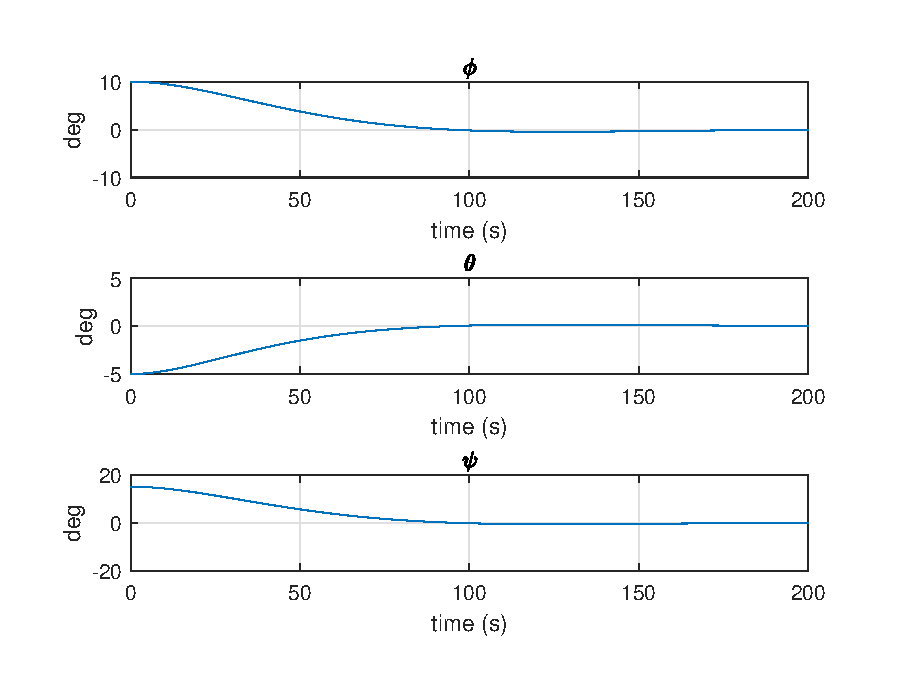
\includegraphics[width=1.00\textwidth]{figures/1_euler.eps}
	\caption{The resulting output Euler angles from the simulation in attitude1.m}
\label{fig:sim_attitude1_euler}
\end{figure}

\begin{figure}[htb!]
	\centering
	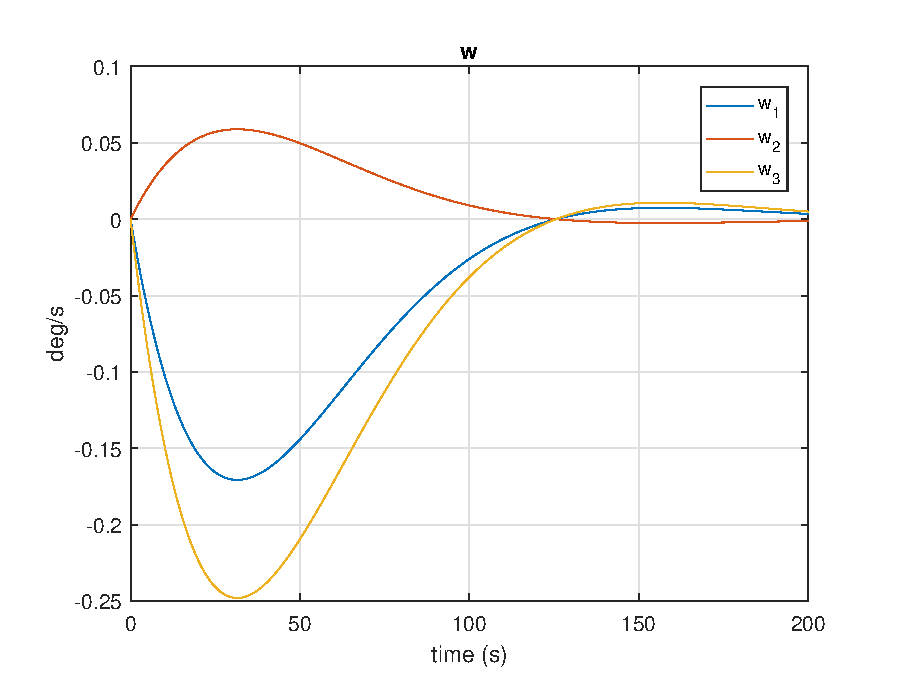
\includegraphics[width=1.00\textwidth]{figures/1_q.eps}
	\caption{The resulting state $x = [\boldsymbol{\eta}^\top, \boldsymbol{\omega}^\top] ^\top$ of the system and $\eta$. $\boldsymbol{\omega}$ is \textbf{w} in the figure. The figure is from the simulation in attitude1.m}
\label{fig:sim_attitude1_q}
\end{figure}

\begin{figure}[htb!]
	\centering
	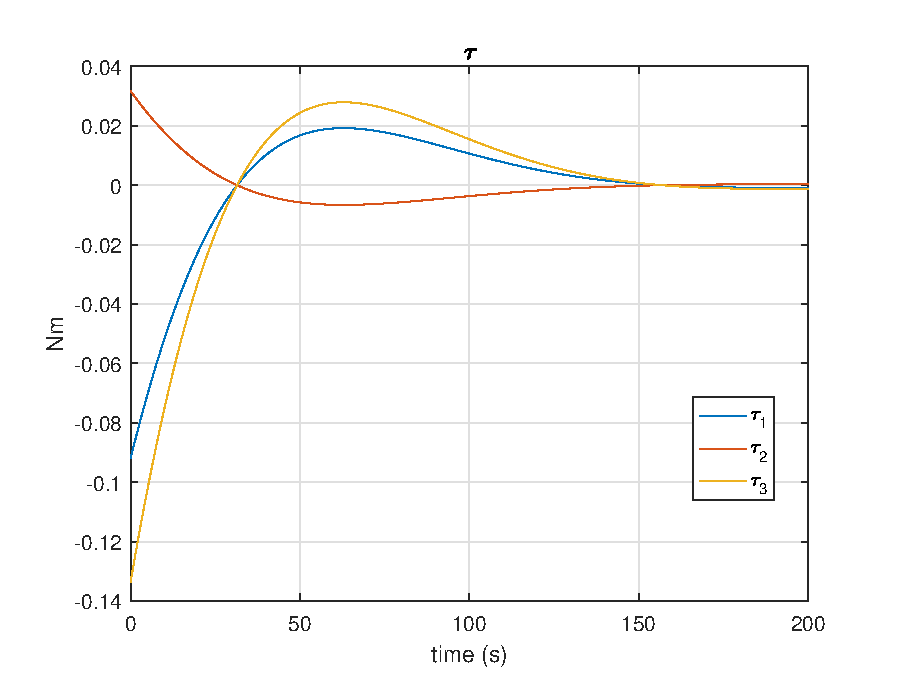
\includegraphics[width=1.00\textwidth]{figures/1_tau.eps}
	\caption{The resulting input $\boldsymbol{\tau}$ from the simulation in attitude1.m}
\label{fig:sim_attitude1_tau}
\end{figure}

The control law implemented in {\color{blue} attitude1.m} implements an  controller which is proportional to the states, meaning it will try to regulate  the states to $\mathbf{0}$. The controller impacts $\boldsymbol{\omega}$ and  $\dot{\mathbf{\eta}}$ is impacted by $\boldsymbol{\omega}$, from equation \eqref{eq:x_dot}.   By looking at Figure \ref{fig:sim_attitude1_euler} - \ref{fig:sim_attitude1_tau}, the steady-state value is zero, meaning the system behaves as expected.

\todo{I don't know if this part should be included}

Looking at the plots it seems as if the unit quaternions and Euler angles reach steady-state before $\boldsymbol{\omega}$. The reason for this may be that the system is 
\todo{I DON'T KNOW!!! Discuss tomorrow when I'm awake}

\todo{Skrives Euler med store eller små bokstaver ?}
\todo{Write htb in front of figures}

\subsection*{Problem 1.4}
A modified attitude control law which controls $\boldsymbol{\eta}$ to a desired value $\mathbf{x}_d = [\boldsymbol{\epsilon}_d^\top \boldsymbol{0}^\top]^\top$ is:

\begin{equation}
    \boldsymbol{\tau} = - \mathbf{K}_d \boldsymbol{\omega} - k_p \tilde{\boldsymbol{\epsilon}}
    \label{eq:control_law_attitude2}
\end{equation}

$\tilde{\boldsymbol{\epsilon}}$ is the error in the imaginary part of the quaternion. The error in the quaternions $\tilde{\mathbf{q}}$ is defined as:

\begin{equation}
    \begin{aligned}
    \tilde{\boldsymbol{q}}
    :=
    \begin{bmatrix}
    \tilde{\boldsymbol{\eta}} \\
    \tilde{\boldsymbol{\epsilon}}
    \end{bmatrix}
    =
    \bar{\boldsymbol{q}}_d \otimes \boldsymbol{q}
    \label{eq:q_tilde}
    \end{aligned}
\end{equation}

with $\bar{q} = [\eta, -\boldsymbol{\epsilon}^\top] ^\top$ and $\mathbf{S}(-\epsilon_d)$ being the skew-symmetric matrix. The quaternion product is defined as :

\begin{equation}
    \bar{\boldsymbol{q}}_d \otimes \boldsymbol{q}
    =
    \begin{bmatrix}
    \boldsymbol{\eta}_{d} \boldsymbol{\eta} + \boldsymbol{\epsilon}_d^\top \boldsymbol{\epsilon} \\
    \boldsymbol{\eta}_d \boldsymbol{\epsilon} - \boldsymbol{\eta} \boldsymbol{\epsilon}_d + \mathbf{S}(-\boldsymbol{\epsilon}_d) \boldsymbol{\epsilon}
    \end{bmatrix}
    \label{eq:q_product}
\end{equation}

\subsubsection*{ Matrix expression for the quaternion error}

The matrix expression for the quaternion error expressed on component form is found by using the equation for quaternion error  \eqref{eq:q_tilde} and the definition of the quaternion product \eqref{eq:q_product}, and is:


\eqref{eq:control_law_attitude3}
\begin{equation}
    \begin{aligned}
    \tilde{\boldsymbol{q}}
    =
    \begin{bmatrix}
    \eta_d \eta + \epsilon_{d,1} \epsilon_1 + \epsilon_{d,2} \epsilon_2 + \epsilon_{d,3} \epsilon_3 \\
    \eta_d \epsilon_1 - \eta \epsilon_{d,1} + \epsilon_{d,3} \epsilon_{2} - \epsilon_{d,2} \epsilon_{3} \\
    \eta_d \epsilon_2 - \eta \epsilon_{d,2} - \epsilon_{d,3} \epsilon_{1} + \epsilon_{d,1} \epsilon_{3} \\
    \eta_d \epsilon_3 - \eta \epsilon_{d,3} + \epsilon_{d,2} \epsilon_{1} - \epsilon_{d,1} \epsilon_{2} \\
    \end{bmatrix}
    \label{eq:q_tilde_full}
    \end{aligned}
\end{equation}

with $\mathbf{q}_d = [\eta_d, \epsilon_{d,1}, \epsilon_{d,2}, \epsilon_{d,3}]^\top$.

\subsubsection*{ Convergence of $\tilde{\mathbf{q}}$}

$\tilde{\mathbf{q}}$ converges means $\mathbf{q} \rightarrow \mathbf{q}_d$. Finding the $\tilde{\mathbf{q}}$ after convergence means setting $\mathbf{q} = \mathbf{q}_d$  in equation \eqref{eq:q_tilde_full} giving:

\begin{equation}
    \begin{aligned}
    \tilde{\boldsymbol{q}}
    =
    \begin{bmatrix}
    \eta \eta + \epsilon_{1} \epsilon_1 + \epsilon_{2} \epsilon_2 + \epsilon_{3} \epsilon_3 \\
    \eta \epsilon_1 - \eta \epsilon_{1} + \epsilon_{3} \epsilon_{2} - \epsilon_{2} \epsilon_{3} \\
    \eta_d \epsilon_2 - \eta \epsilon_{2} - \epsilon_{3} \epsilon_{1} + \epsilon_{1} \epsilon_{3} \\
    \eta \epsilon_3 - \eta \epsilon_{3} + \epsilon_{2} \epsilon_{1} - \epsilon_{1} \epsilon_{2} \\
    \end{bmatrix}
    = 
    \begin{bmatrix}
    1 \\
    0\\
    0 \\
    0 \\
    \end{bmatrix}
    \label{eq:q_con}
    \end{aligned}
\end{equation}

The result from equation \eqref{eq:q_con} is that the error of the quaternions will converge to zero for $\boldsymbol{\epsilon}$. The reason for $\eta$ not converging to zero, is the constraint of unit quaternions, which states $\eta \eta + \epsilon_1 \epsilon_1 + \epsilon_2 \epsilon_2 + \epsilon_3 \epsilon_3 = 0$. 

\todo{Should I say anything more ?}



